% !TEX root = main.tex
% Main text: abstract through conclusion. Formal assumptions, full statements and proofs are in the appendix.
\begin{abstract}
Running states expose gradient information that final counts hide.
For modular counting, both direct and step-by-step programs fit in the same
two-block Transformer. A contraction coefficient $\lambda$ suppresses outcome
credit on the scale $\lambda^n$, while displayed states retain local innovation
controlled by $1-\lambda^2$. A Transformer score expansion yields quantitative
credit bounds and an exponentially long outcome-training plateau near small
initialization. An aligned structured Transformer learns the recurring process transitions in
polynomial time with supplied routing and a restricted trained family.
In a reduced two-path model containing both exact executors,
a small initial loss gap keeps outcome gradient flow in an affine activation
region and forces convergence to a suboptimal minimum under an explicit
geometric condition. A separate exact symmetric seed gives polynomial process
learning and permanent outcome failure. Experiments test the initialization
boundary, routing, supervision budget and transfer; an object-tracking reversal
shows that low-degree signal alone does not predict optimization.
\end{abstract}

% ===================================================================
\section{Introduction}
\label{sec:intro}

A final-answer algorithm and a step-by-step algorithm can both fit inside one Transformer,
yet gradient training can reach them at very different speeds. We isolate this optimization
question using modular counting. Proposition~\ref{prop:represent} constructs exact executors
for both formats in the same two-block architecture. Intermediate supervision is known to
help reasoning \citep{nye2021scratchpads,wei2022cot,lightman2023verify}; here we trace its
benefit through the statistical information in a label, gradient credit and outcome training time.

\paragraph{Optimization obstruction despite expressibility.}
Both exact counting programs exist in the architecture, but their existence does
not ensure that training reaches them. Under its small-initialization hypotheses,
Theorem~\ref{thm:outcome-end} bounds the outcome plateau by
$T_{\mathrm{out}}\ge c\lambda^{-n}$. Theorem~\ref{thm:separation} shows that
step labels retain local rule credit. The aligned structured reduction separately
proves polynomial transition learning (\cref{thm:aligned-transformer}); this
positive guarantee retains fixed feature roles and supplied routing.
A matched process-convergence result is proved separately for an exact symmetric
seed of the reduced two-path family (\cref{prop:two-path-matched}).
A separate reduced model gives an attracting suboptimal outcome minimum despite
containing an exact outcome executor (\cref{prop:two-path-trap}).

\paragraph{Mechanism and scope.}
Each unseen letter contracts a feature's final-count correlation by $\lambda<1$.
Small initialization makes terms that read few letters dominate the gradient;
displaying the previous state exposes a local innovation instead.
The full-network plateau requires small initialization, zero readout and MLP
biases bounded away from zero after normalization. The two-path trap supplies
routing and count averaging, and its random-seed certificate applies only above a quantitative horizon
threshold. Process convergence from the same nonsymmetric seeds is unproved. Initializing its ReLU kinks in range allows outcome training
to cross high accuracy (\cref{app:two-path}). Empirical tests extend beyond these regimes.

\begin{figure}[t]
\centering
%% Figure 1 (pgfplots). Data: results/paper/zero_readout_n16_8k (seeds 42-51, median and 25th-75th percentile band),
%% results/paper/fig2/n8_s42.json (target A_r) and results/paper/exact_spectra/sigma_sweep/s42_sg0.02.txt (Jacobian J_r).
\definecolor{stepc}{HTML}{0072B2}\definecolor{outc}{HTML}{D55E00}\definecolor{theoc}{HTML}{009E73}
\definecolor{modelc}{HTML}{7B4F9E}\definecolor{mutedc}{HTML}{6E6E6E}
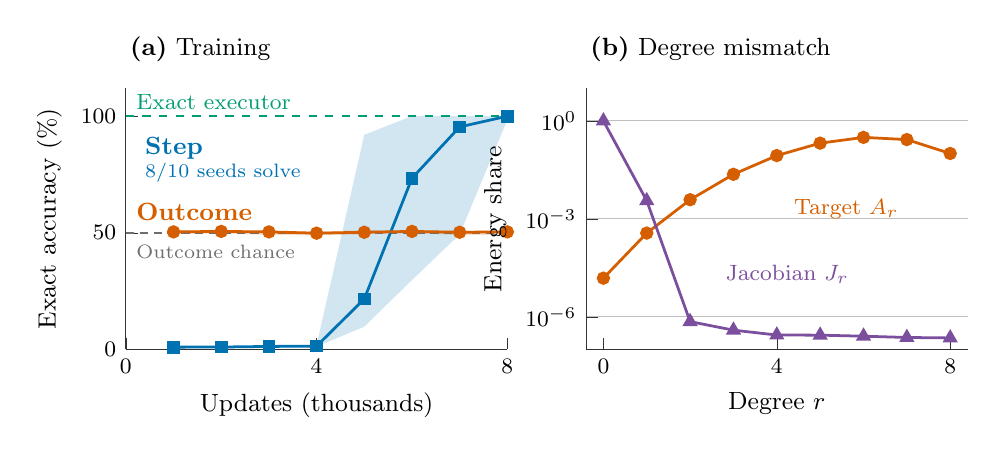
\begin{tikzpicture}
\pgfplotsset{every axis/.style={width=0.53\linewidth, height=4.9cm, axis line style={black!80}, tick style={black!80},
  tick label style={font=\footnotesize}, label style={font=\small}, title style={font=\small, at={(0,1)}, anchor=south west, xshift=-2pt}},
  every axis plot/.append style={line width=1pt}}
\begin{axis}[name=train, title={\textbf{(a)} Training}, xlabel={Updates (thousands)}, ylabel={Exact accuracy (\%)},
  xmin=0, xmax=8, ymin=0, ymax=112, xtick={0,4,8}, ytick={0,50,100}, axis x line*=bottom, axis y line*=left, clip=false]
  \addplot[draw=none, fill=stepc, fill opacity=0.18, forget plot] coordinates {(1,0.55) (2,0.73) (3,0.82) (4,1.25) (5,9.77) (6,29.75) (7,49.33) (8,98.40) (8,100.00) (7,100.00) (6,100.00) (5,92.03) (4,1.90) (3,1.40) (2,1.35) (1,1.35)};
  \addplot[draw=none, fill=outc, fill opacity=0.18, forget plot] coordinates {(1,49.52) (2,49.73) (3,49.05) (4,48.92) (5,49.35) (6,49.92) (7,48.97) (8,49.15) (8,50.70) (7,50.70) (6,51.20) (5,51.08) (4,50.60) (3,50.70) (2,51.08) (1,51.08)};
  \addplot[theoc, dashed, line width=0.9pt, domain=0:8, samples=2] {100};
  \addplot[mutedc, densely dashed, line width=0.8pt, domain=0:8, samples=2] {50};
  \addplot[stepc, mark=square*, mark size=1.8pt] coordinates {(1,1.00) (2,1.05) (3,1.30) (4,1.45) (5,21.65) (6,73.40) (7,95.40) (8,100.00)};
  \addplot[outc, mark=*, mark size=1.9pt] coordinates {(1,50.40) (2,50.60) (3,50.40) (4,49.85) (5,50.25) (6,50.60) (7,50.25) (8,50.40)};
  \node[anchor=south west, font=\footnotesize, text=theoc, inner sep=1pt] at (axis cs:0.15,101.5) {Exact executor};
  \node[anchor=west, font=\small\bfseries, text=stepc] at (axis cs:0.2,86) {Step};
  \node[anchor=west, font=\scriptsize, text=stepc] at (axis cs:0.2,76) {8/10 seeds solve};
  \node[anchor=south west, font=\small\bfseries, text=outc, inner sep=1pt] at (axis cs:0.15,54) {Outcome};
  \node[anchor=north west, font=\scriptsize, text=mutedc, inner sep=1pt] at (axis cs:0.15,46) {Outcome chance};
\end{axis}
\begin{semilogyaxis}[at={(train.east)}, anchor=west, xshift=1.0cm, title={\textbf{(b)} Degree mismatch}, xlabel={Degree $r$},
  ylabel={Energy share}, xmin=-0.4, xmax=8.4, ymin=1e-7, ymax=10, xtick={0,4,8}, ytick={1e-6,1e-3,1},
  ymajorgrids, major grid style={black!25}, axis x line*=bottom, axis y line*=left]
  \addplot[outc, mark=*, mark size=1.9pt] coordinates {(0,1.5259e-05) (1,3.6621e-04) (2,3.8452e-03) (3,2.3071e-02) (4,8.6517e-02) (5,2.0764e-01) (6,3.1146e-01) (7,2.6697e-01) (8,1.0011e-01)};
  \addplot[modelc, mark=triangle*, mark size=2.2pt] coordinates {(0,9.9641e-01) (1,3.5840e-03) (2,7.1281e-07) (3,3.9081e-07) (4,2.7680e-07) (5,2.7450e-07) (6,2.5510e-07) (7,2.3310e-07) (8,2.2560e-07)};
  \node[anchor=north, font=\footnotesize, text=outc] at (axis cs:5.6,8e-3) {Target $A_r$};
  \node[anchor=west, font=\footnotesize, text=modelc] at (axis cs:2.6,2e-5) {Jacobian $J_r$};
\end{semilogyaxis}
\end{tikzpicture}

\caption{\textbf{Same architecture and task, different training behavior.}
(a)~Counting with $n=16$, $K=2$ and zero readout: median exact continuation accuracy and interquartile band over ten paired seeds, $8$k
updates; the dashed line marks the exact executor that both formats admit (\cref{prop:represent}).
(b)~A separate $n=8$, $K=2$, $\initscale=0.02$ measurement with nonzero readout: target and Jacobian energy occupy different interaction degrees, defined by the number of letters a component depends on jointly (\cref{app:spectrum}).}
\label{fig:overview}
\end{figure}

\needspace{3\baselineskip}
\paragraph{Contributions.}
\begin{itemize}[leftmargin=*,itemsep=3pt,topsep=3pt]
\item \textbf{A data-to-gradient mechanism.} Fourier contraction and a Transformer
score expansion quantify hidden outcome credit; displayed states retain local rule
credit (\cref{thm:main,thm:separation}).
\item \textbf{Optimization obstructions despite expressibility.} Both formats admit
exact executors. We prove a full-network outcome plateau, aligned structured
transition convergence, and certified two-path outcome traps
(\cref{prop:represent,thm:outcome-end,thm:aligned-transformer,prop:random-outcome-trap}).
\item \textbf{Empirical tests.} We measure prior fitting, rule learning, joint routing
and transfer, including an object-tracking reversal (\cref{sec:experiments}).
\end{itemize}

% ===================================================================
\section{Setup}
\label{sec:setup}
\label{sec:setting}

Modular counting keeps the state space fixed as the prompt grows. What increases is the number of updates hidden behind the
answer. We can therefore lengthen the computation without changing the prediction problem at its end.

\begin{definition}[Counting modulo $K$]
\label{def:task}
A prompt has a start count $s_0$, uniform on $\mathbb Z_K$, and letters $w_1,\ldots,w_n$ drawn i.i.d.\ from an alphabet
in which a fixed query letter $w^\star$ has probability $p\in(0,1)$. With $b_t=\mathbf 1[w_t=w^\star]$,
\begin{equation}
 s_t=s_{t-1}+b_t\pmod K,\qquad t=1,\ldots,n,
 \label{eq:tracking}
\end{equation}
and the answer is $y=s_n$.
\end{definition}

\begin{definition}[Contraction coefficient]
\label{def:lambda}
For counting modulo $K$,
\begin{equation}
 \mixrate=\max_{1\le j<K}\bigl|1-p+p\,e^{2\pi\mathrm ij/K}\bigr|=\bigl|1-p+p\,e^{2\pi\mathrm i/K}\bigr|.
 \label{eq:lambda}
\end{equation}
\end{definition}

\begin{figure}[t]
\centering
\resizebox{\linewidth}{!}{% Conceptual figure: counting modulo K as a cyclic chain, and what each supervision format sees.
\begin{tikzpicture}[>=Stealth, font=\small,
  state/.style={circle, draw=royalazure!80!black, fill=royalazure!12, minimum size=7mm, inner sep=0pt},
  tok/.style={rectangle, rounded corners=2pt, draw=black!45, fill=black!4, minimum width=7mm, minimum height=5.5mm, inner sep=1pt},
  sup/.style={rectangle, rounded corners=2pt, draw=royalazure!80!black, fill=royalazure!12, minimum width=7mm, minimum height=5.5mm, inner sep=1pt},
  hid/.style={rectangle, rounded corners=2pt, draw=black!30, dashed, fill=white, text=black!45, minimum width=7mm, minimum height=5.5mm, inner sep=1pt}]

% ---------------- (a) cyclic chain ----------------
\begin{scope}[shift={(0,0)}]
  \foreach \i/\lab in {0/0, 1/1, 2/2, 3/{K{-}1}} {
    \node[state] (c\i) at ({90-\i*90}:1.25) {$\lab$};
  }
  \foreach \i/\dir in {0/90, 1/0, 2/-90, 3/180} {
    \draw[->, black!55] (c\i) to[out=\dir+28, in=\dir-28, looseness=6] node[pos=0.5, font=\scriptsize, fill=white, inner sep=0.5pt] {$1{-}p$} (c\i);
  }
  \draw[->, thick, royalazure] (c0) to[bend left=22] node[font=\scriptsize, above right=-1pt] {$p$} (c1);
  \draw[->, thick, royalazure] (c1) to[bend left=22] node[font=\scriptsize, below right=-1pt] {$p$} (c2);
  \draw[->, thick, royalazure, dashed] (c2) to[bend left=22] node[font=\scriptsize, below left=-1pt] {$p$} (c3);
  \draw[->, thick, royalazure] (c3) to[bend left=22] node[font=\scriptsize, above left=-1pt] {$p$} (c0);
  \node[align=center, font=\footnotesize] at (0,-2.6)
    {$s_t=s_{t-1}+b_t\ (\mathrm{mod}\ K)$\\[2pt] $\mathbf T=(1-p)\,\mathbf I+p\,\mathbf R$};
  \node[font=\small\bfseries] at (-2.3,1.75) {(a)};
\end{scope}

% ---------------- (b) what each format supervises ----------------
\begin{scope}[shift={(3.4,0.95)}]
  \node[font=\small\bfseries] at (-0.35,0.8) {(b)};
  % outcome row
  \node[anchor=west, font=\footnotesize] at (0,0.8) {Outcome: supervise $s_n$ only};
  \node[tok] (o0) at (0.45,0) {$s_0$};
  \node[tok] (ow1) at (1.35,0) {$w_1$};
  \node[hid] (os1) at (2.25,0) {$s_1$};
  \node[tok] (ow2) at (3.15,0) {$w_2$};
  \node[hid] (os2) at (4.05,0) {$s_2$};
  \node at (4.85,0) {$\cdots$};
  \node[tok] (own) at (5.65,0) {$w_n$};
  \node[sup] (osn) at (6.55,0) {$s_n$};
  \draw[decorate, decoration={brace, amplitude=4pt, mirror}, black!60] (1.0,-0.42) -- (6.0,-0.42)
    node[midway, below=4pt, font=\footnotesize, align=center] {$n$ hidden letters: each Fourier mode contracts by $\le\mixrate$ per letter};
  % step row
  \node[anchor=west, font=\footnotesize] at (0,-1.75) {Step: supervise every $s_t$ from the displayed $s_{t-1}$};
  \node[tok] (p0) at (0.45,-2.55) {$s_0$};
  \node[tok] (pw1) at (1.35,-2.55) {$w_1$};
  \node[sup] (ps1) at (2.25,-2.55) {$s_1$};
  \node[tok] (pw2) at (3.15,-2.55) {$w_2$};
  \node[sup] (ps2) at (4.05,-2.55) {$s_2$};
  \node at (4.85,-2.55) {$\cdots$};
  \node[tok] (pwn) at (5.65,-2.55) {$w_n$};
  \node[sup] (psn) at (6.55,-2.55) {$s_n$};
  \draw[rounded corners=3pt, thick, lightmauve!80!black] (1.83,-2.95) rectangle (3.55,-2.15);
  \draw[->, thick, lightmauve!80!black] (3.55,-2.55) -- (ps2.west);
  \node[font=\footnotesize, align=center] at (3.5,-3.45) {one local transition $(s_{t-1},w_t)\mapsto s_t$: innovation $\ge1-\mixrate^2$};
\end{scope}
\end{tikzpicture}
}
\caption{\textbf{One counting process, two views of it.}
(a)~Counting modulo $K$ is a cyclic Markov chain: each letter keeps the count with probability $1-p$ and advances it with probability
$p$, so the transition matrix is $\mathbf T=(1-p)\mathbf I+p\mathbf R$ with $\mathbf R$ the cyclic shift. Its nonconstant Fourier modes
contract by at most $\mixrate$ per step (\cref{app:contraction}).
(b)~Outcome supervision labels only $s_n$, so the label depends on the letters through $n$ unseen steps of the chain and its
correlation with any feature of $k$ letters shrinks like $\mixrate^{n-k}$ (\cref{thm:main}). Step supervision displays $s_{t-1}$ and labels $s_t$, so each label is one
step of the chain and keeps an innovation of at least $1-\mixrate^2$ (\cref{thm:separation}).}
\label{fig:chain}
\end{figure}

Averaging over one unseen letter contracts every nonconstant Fourier mode of the count by at most $\mixrate$ (\cref{fig:chain}); in information-theoretic terms,
$\mixrate$ is the maximal correlation of consecutive counts and $\mixrate^2$ the chi-squared contraction coefficient of one
unseen letter \citep{witsenhausen1975sequences,raginsky2016strong}.
The same descriptor controls the final-answer scale $\lambda^n$ and the
normalized Fourier innovation $1-\lambda^2$ (\cref{eq:move-variance}); for general
$K$, the state-innovation covariance is bounded below by
$(1-\lambda^2)/K$ on the centered state subspace (\cref{eq:local-variation}).
For four uniform letters,
$\mixrate=0.5$ at $K=2$ and $0.66$ at $K=3$.

\paragraph{Formats.} Both formats see the same prompt. The \emph{outcome loss} $\Lout$ is the cross-entropy of the final
count; the \emph{step loss} $\Lstep$ is the teacher-forced cross-entropy of the transitions $s_{t-1},w_t\mapsto s_t$ for
$t\ge2$; the first prediction is a boundary case whose previous count sits in the prompt (\cref{def:losses}). Experiments
supervise every running count unless stated otherwise.

\paragraph{Model.} Two causal attention/ReLU blocks without LayerNorm, with a linear readout,
contain exact solutions for both formats. The credit and plateau results use small initialization
with a fixed local ReLU pattern; \cref{ass:arch,ass:init} specify the norm, bias and conditioning
requirements. Experiments also test training beyond this regime.

\begin{proposition}[Both solutions exist]
\label{prop:represent}
For every $K$, alphabet size and $n$, one architecture as in \cref{ass:arch}, with widths linear in $n$, has parameters
$\thstep$ and $\thout$ at which greedy decoding produces the correct step and outcome continuations on every prompt, with
a positive logit margin.
\end{proposition}

The step executor retrieves the previous state and current match bit before a modular lookup;
the outcome executor aggregates match bits before the lookup. Both use constant depth and width
linear in the horizon. Their tensor entries and positive margins are proved in \cref{app:architectures}.

% ===================================================================
\section{Credit through unseen letters}
\label{sec:credit}

To understand the training gap, we first ask how much information about the target reaches a parameter update.
Fix the start count, so the letters are independent.

\begin{definition}[Credit]
\label{def:credit}
For a target signal $\bm\xi$, a random vector in $\R^K$, let $\cred_{\bm\xi}(\bm\theta)=\E[\langle\bm z_{\bm\theta},\bm\xi\rangle]$. The
\emph{credit} for $\bm\xi$ is $\|\nabla_{\bm\theta}\cred_{\bm\xi}\|=\bigl\|\E\bigl[(\Jz)^\top\bm\xi\bigr]\bigr\|$.
\end{definition}

For the outcome signal $\bm\xi=\bm y-\bm u$ (one-hot answer minus uniform), credit is the answer-dependent part of the gradient of
$\Lout$ (\cref{lem:gradient-split}; \citealp{shalevshwartz2017failures,abbe2025parities}).

\subsection{Outcome: few-letter features cannot see the final count}
\paragraph{What a feature misses.} Suppose a feature $\mathbf H$ reads only the letters in a set $S$. Even if it uses those letters perfectly,
it must average over every letter outside the set. By the tower property,
$\E[\mathbf H^\top(\bm y-\bm u)]=\E[\mathbf H^\top\E[\bm y-\bm u\mid w_S]]$, and given $w_S$ the $n-|S|$ unseen letters still move the count: each
multiplies every nonconstant Fourier mode of its distribution by at most $\mixrate$ (\cref{fig:chain}a). Hence
\begin{equation}
 \bigl\|\E\bigl[\mathbf H^\top(\bm y-\bm u)\bigr]\bigr\|\le\mixrate^{n-|S|}\,\|\mathbf H\|_{L^2}
 \label{eq:credit-degree}
\end{equation}
(\cref{lem:target-contraction}). Each omitted letter has the same multiplicative cost; seeing a few letters cannot bypass the rest of
the computation. The exponent is sharp.

\paragraph{The network reads few letters at a time.} Scale every attention score by $\zeta\in[0,1]$ and expand in $\zeta$. At $\zeta=0$ attention is uniform
and the MLPs are affine, so the network is additive over positions: each term reads at most one letter. Every interaction among letters
passes through the scores, and a term with $k\ge1$ scores reads at most $2k+1$ letters and costs $\initscale^{2+4k}$ in the Jacobian
(\cref{prop:score-degree}). Applying \cref{eq:credit-degree} term by term bounds the outcome credit. Call the credit of the score-dependent part
$\mathbf J_{\mathrm{score}}$ of the Jacobian the \emph{score-mediated credit}: it contains every term that reads two or more letters, and
also score-dependent terms that read one.

\begin{theorem}[Unseen letters erase outcome credit]
\label{thm:main}
Under \cref{ass:arch,ass:init,ass:task}, with the start count fixed:
\begin{enumerate}[label=(\roman*),leftmargin=*,itemsep=0pt,topsep=2pt]
\item for every set $S$ of letters and every square-integrable $\mathbf H$ that depends only on the letters in $S$, \cref{eq:credit-degree} holds;
\item for all $n\ge2$, $\initscale^2\le c\mixrate$ and $\bm\theta\in\initball$, the score-mediated credit is at most $C\initscale^6\mixrate^{n-3}$, and if
$\initscale\le c\mixrate$ the whole outcome credit is at most $C\initscale\mixrate^n$.
\end{enumerate}
\end{theorem}

\paragraph{An exact binary loss identity.}
For a predictor that reads the displayed initial state and one letter, the contraction
appears directly in the loss. This identity applies to that restricted predictor, not
to a count-reading path or the full Transformer.
\begin{lemma}[One-letter binary loss identity]
\label{lem:binary-loss-mixture}
Let $K=2$, $0<p<1/2$, and $\lambda=1-2p$. Let $S$ be uniform on
$\{-1,1\}$, independently of the letters, and put $C_j=(-1)^{b_j}$.
For any differentiable predictor $f_\theta(S,C_n)$, define
\[
\begin{aligned}
 L_{\mathrm{step}}^{\mathrm{gate}}&=\E\bigl[\ell(SC_n f_\theta(S,C_n))\bigr],\\
 L_{\mathrm{out}}^{\mathrm{gate}}&=\E\bigl[\ell(S\textstyle\prod_{j=1}^n C_j\, f_\theta(S,C_n))\bigr],\\
 L_{\mathrm{sym}}^{\mathrm{gate}}&=\tfrac12\E\bigl[\ell(f_\theta(S,C_n))+\ell(-f_\theta(S,C_n))\bigr],
 \qquad \ell(u)=\log(1+e^{-u}).
\end{aligned}
\]
Then
\begin{equation}
 L_{\mathrm{out}}^{\mathrm{gate}}
 =L_{\mathrm{sym}}^{\mathrm{gate}}
 +\lambda^{n-1}\bigl(L_{\mathrm{step}}^{\mathrm{gate}}-L_{\mathrm{sym}}^{\mathrm{gate}}\bigr).
 \label{eq:binary-loss-mixture}
\end{equation}
The same identity holds after applying $\nabla_\theta$.
\end{lemma}
\begin{proof}
The hidden product $H=\prod_{j<n}C_j$ is independent of $(S,C_n)$, with
$\Pr(H=\pm1)=(1\pm\lambda^{n-1})/2$. Thus
\[
 L_{\mathrm{out}}^{\mathrm{gate}}
 =\tfrac{1+\lambda^{n-1}}2 L_{\mathrm{step}}^{\mathrm{gate}}
 +\tfrac{1-\lambda^{n-1}}2
 \E[\ell(-SC_n f_\theta(S,C_n))].
\]
The two signed losses sum to $2L_{\mathrm{sym}}^{\mathrm{gate}}$.
Differentiation commutes with these finite expectations.
\end{proof}
The excess over the symmetric-label loss is attenuated by $\lambda^{n-1}$.
This identifies a loss mechanism; a predictor restricted to these inputs cannot
express the outcome executor, so the identity alone is not an optimization separation.

\subsection{Step: a local innovation survives}
A large step gradient could be misleading. The displayed count alone predicts the two possible next states and their probabilities.
Fitting that prior lowers the loss without learning how to use the current letter. We separate that easy signal from the rule itself. With the
state-only predictor $\bm q_s=(1-p)\bm e_s+p\,\bm e_{s+1}$, write $\bm e_{s_t}-\bm u=(\bm q_{s_{t-1}}-\bm u)+\bm g_t$, where the
\emph{rule signal}
\[
 \bm g_t=\bm e_{s_t}-\bm q_{s_{t-1}}=(b_t-p)\bigl(\bm e_{s_{t-1}+1}-\bm e_{s_{t-1}}\bigr)
\]
has covariance, on the centred state subspace $\one^\perp:=\{v\in\R^K:\one^\top v=0\}$,
\begin{equation}
 \operatorname{Cov}(\bm g_t)\succeq\frac{1-\mixrate^2}{K}\,I
 \quad\text{on }\one^\perp.
 \label{eq:local-variation}
\end{equation}
Thus an outcome target pays $\mixrate^{n-|S|}$ for the letters a feature does not read, whereas a displayed transition pays the
local innovation $1-\mixrate^2$ only once. Let $\rulecredit$ be the credit
functional with the rule signal as target.

\begin{theorem}[Step credit]
\label{thm:separation}
For parts (i)--(ii), under \cref{ass:arch,ass:init,ass:task} with a uniform start,
for all $n\ge2$ and $\bm\theta\in\initball$:
\begin{enumerate}[label=(\roman*),leftmargin=*,itemsep=0pt,topsep=2pt]
\item \emph{(prior-fitting gradient)} if $\initscale\le c\mixrate$, then $\|\nabla_{\bm\theta}\Lstep(\bm\theta)\|\ge c\,\initscale\mixrate$ while
$\|\nabla_{\bm\theta}\Lout(\bm\theta)\|\le C\initscale(\initscale^2+\mixrate^n)$;
\item \emph{(rule credit)} if $\initscale\le c$ and attention uses the full causal prefix, then $\|\nabla_{\bm\theta}\rulecredit(\bm\theta)\|\le \frac{C\initscale^6}{n}$; if
moreover $p<\tfrac{1}{2}$, the degree-$6$ polynomial $P_n$ is not identically zero, with an explicit count$\times$letter monomial of
coefficient of order $\frac{1}{n\sqrt{d_{\mathrm h}}}$
(\cref{lem:leading}).
\input{sections/thm2_gaussian_statement}
\end{enumerate}
\end{theorem}

Part~(i) fits the state-only prior; part~(ii) isolates the local rule signal.
Part~(iii) turns generic nonvanishing into a sufficiently-small-scale Gaussian rule-credit
lower bound under a quantitative geometry event. \Cref{app:t2-gaussian-geometry}
verifies an explicit Gaussian-weight law with nonzero bias magnitudes. This is an initial
rule-credit statement, not a full cross-entropy-gradient or training-time bound.

% ===================================================================
\section{Which solution training reaches}
\label{sec:reach}

Small initial credit alone does not imply slow learning: the parameters might reach a region with a stronger signal. We ask
whether outcome flow can get there quickly. We then exhibit an attracting outcome trap in a reduced family with both executors.

\subsection{Outcome: an exponential plateau}

The next theorem controls the trajectory as it tries to leave initialization. A local loss floor limits how far gradient flow can travel.

\begin{theorem}[Exponential-time outcome plateau near small initialization]
\label{thm:outcome-end}
Under \cref{ass:arch,ass:init,ass:task} with a zero initial readout, let $P(t)$ be, at each time, the orthogonal projection onto a set
of trainable parameter blocks, piecewise constant in $t$; the blocks may include the relative bias. Consider gradient flow
$\tfrac{d\bm\theta}{dt}=-\mathbf P(t)\nabla_{\bm\theta}\Lout(\bm\theta)$; full joint flow ($\mathbf P\equiv\mathbf I$) and training a fixed subset of blocks are special cases.
For all $n\ge2$, $\initscale\le c\mixrate$ and $0\le t\le c\mixrate^{-n}$, with constants that do not depend on the schedule:
\begin{enumerate}[label=(\roman*),leftmargin=*,itemsep=0pt,topsep=2pt]
\item \emph{(locality)} $\|\bm\theta(t)-\bm\theta_0\|\le\ballradius\initscale$, the relative bias included in the norm;
\item \emph{(loss)} $\Lout(\bm\theta(t))\ge\log K-C\initscale^2\mixrate^n$;
\item \emph{(correct-answer probability)} $\E\bigl[\softmax(\bm z_{\bm\theta(t)})_y\bigr]\le\frac{1}{K}+C\initscale\mixrate^{n/2}$.
\end{enumerate}
\end{theorem}
The theorem bounds the length of the plateau; it does not assert that outcome training never converges.

\emph{Proof idea.} Along the flow, for any schedule,
\[
 \frac{d\Lout}{dt}=-\|\mathbf P(t)\nabla_{\bm\theta}\Lout\|^2,
 \qquad\text{so}\qquad
 \|\bm\theta(t)-\bm\theta_0\|^2\le t\,\bigl(\Lout(\bm\theta_0)-\Lout(\bm\theta(t))\bigr).
\]
This gives the weak signal a consequence beyond the first update. Near $\bm\theta_0$, the outcome loss can fall by at most
$C\initscale^2\mixrate^n$ (\cref{lem:score-sum}), even with a trained relative bias (\cref{lem:bias-uniform}). That small decrease limits
the distance the flow can travel: leaving the ball takes time of order $\mixrate^{-n}$ (\cref{app:end}).

\subsection{Aligned structured Transformer learning}
\label{sec:aligned-transformer}
An exact Transformer reduction supplies the positive convergence result.
The routing mask and feature registers are prescribed; readouts and query--key
maps train jointly in their matrix Frobenius metric.
\begin{theorem}[Aligned process learning and matched outcome time bounds]
\label{thm:aligned-transformer}
Use the structured seed and matrix subspaces of \cref{app:aligned-seed}, with
$K\ge2$, $p\in(0,1)\setminus\{1/2\}$, uniform start, $0<\varepsilon\le1/2$,
zero readouts, $\varepsilon/2\le|q_0|,|k_0|,|v|\le2\varepsilon$ and
$q_0k_0(1-2p)<0$. Process-supervised Euclidean matrix gradient flow learns
every transition at $t\ge2$ with persistent positive margins and
$L_{\mathrm{step}}\to0$ by
\[
 T_{\mathrm{process}}\le
 \frac{410112K d_h\log K}{p_{\min}^2\varepsilon^{12}},
 \qquad p_{\min}=\min(p,1-p).
\]
If $\varepsilon$ also meets the small-initialization conditions of
\cref{thm:outcome-end}, outcome flow from the same seed, mask and trained
matrix subspaces stays near initialization with near-chance correct-answer
probabilities for $T_{\mathrm{outcome}}\ge c\lambda^{-n}$.
At executor widths $d_h,w=\Theta(n)$ and $\varepsilon=c_0n^{-1/2}$, with $c_0$
sufficiently small and fixed $K,p$ and alphabet, these bounds are polynomial $O(n^7)$
and exponential respectively.
\end{theorem}
The proof is the short chain of exact features, symmetry, an aligned gate
invariant and global descent in \cref{app:aligned-transformer}.
The learned transitions are the recurring process computation; a correct first
state, formatting and final-answer copy are separate boundary operations.
The comparison uses a restricted trained family that does not contain the
exact outcome executor. Proposition~\ref{prop:represent} establishes expressibility
in the ambient architecture; the two-path model below supplies same-family
expressibility. These are distinct guarantees.

\subsection{An explicit optimization trap despite exact representability}
\label{sec:two-path-trap}
A reduced family separates missing capacity from an activation trap. For binary
counting, put $S=(-1)^{s_{\mathrm{prev}}}$, $C=(-1)^{b_{\mathrm{gate}}}$,
and let $u$ be the mean bit value in a supplied averaging mask. Let $P$ collect all trainable parameters in
\begin{equation}
 f_P(S,C,u)=S\bigl(a+g\tanh(qk)C\bigr)
 +\sum_{i=1}^{6(n+1)}v_i\relu(w_i u+d_iS+b_i).
 \label{eq:two-path-model}
\end{equation}
At transition $t$, the inputs are $s_{t-1}$, $b_t$ and the mean of the first
$t$ bits; at the answer they are $s_0$, $b_n$ and the mean of all bits.
The masks are supplied by position; only the supervised objective changes.

\begin{proposition}[An attracting suboptimal outcome minimum]
\label{prop:two-path-trap}
For $n\ge2$, $0<p<1/2$ and a uniform start, the family in
\cref{eq:two-path-model} contains positive-margin executors for both formats.
Nevertheless, its population outcome logistic loss has a non-strict local minimum
with
\[
 f_{\mathrm{trap}}(S,C,u)=S C\log\frac{1+\lambda^{n-1}}{1-\lambda^{n-1}},
 \qquad \Pr(Yf_{\mathrm{trap}}>0)=\frac{1+\lambda^{n-1}}2<1.
\]
There is an open neighborhood of a constructed minimum from which full
Euclidean outcome gradient flow keeps its ReLU pattern fixed and converges
to a minimum with these logits, although the family's global loss infimum is zero.
\end{proposition}
The proof in \cref{app:two-path} uses convexity in four effective coefficients
and a local path-length bound in the original parameters. The neighborhood is
around the constructed minimum. Proposition~\ref{prop:random-outcome-trap}
extends trapping to sufficiently small-gap zero-readout seeds. In nine paired fixed-pattern runs, steps solve in $11$--$15$ updates while
outcome runs end at the one-letter accuracy above. Initializing kinks in range
lets all nine outcome runs cross $90\%$ accuracy, sometimes transiently
(\cref{fig:two-path-init}). This reduced trap complements the full-network plateau
of \cref{thm:outcome-end}; the low-horizon experimental seeds remain uncertified.

\paragraph{A trap without freezing the count path.}
An exponentially small initial loss gap also controls trajectories with nonzero
averaging state weights.
\begin{proposition}[Outcome trapping from zero readout]
\label{prop:random-outcome-trap}
Let $n\ge2$, $0<p<1/2$ and the start be uniform. In \cref{eq:two-path-model},
initialize $a=g=v_i=0$. Suppose each ReLU is active for all inputs or inactive for all inputs,
and the seed satisfies the computable geometry certificate of
\cref{app:random-trap-certificate}, with radius $r$ and bounds
$c_{\mathrm{map}},c_{\mathrm{loss}}>0$. If
\[
 \frac{\sqrt2\lambda^{n-1}}{c_{\mathrm{map}}\sqrt{c_{\mathrm{loss}}}}<\frac r2,
\]
full Euclidean outcome gradient flow remains in that activation region and
converges to a suboptimal local minimum with logits $f_{\mathrm{trap}}$.
Its loss is at least $L_{\mathrm{trap}}$ throughout; its limiting accuracy is
$(1+\lambda^{n-1})/2$. The state weights $d_i$ need not vanish.
\end{proposition}
The seed's loss gap above the affine minimum is at most $\lambda^{2(n-1)}$.
The coefficient Hessian has a quantitative lower bound proportional to $1/n$,
and a gradient lower bound turns that gap into a finite parameter path length.
For the initialization law used in Figure~\ref{fig:two-path-init}, the certificate
first passes at $n=17,17,16$ for seed streams $0,1,2$ at $\varepsilon=0.3$.
These are checked draws at varying widths, not a uniform guarantee over all
later draws; the $n=4$--$8$ simulations remain below the certified threshold.
The distribution-wide bound of \cref{cor:random-trap-geometry} applies at $n=25$
with probability at least $0.9448$ for these $p,\varepsilon$.

\paragraph{Complementary matched two-path flows.}
For an exact symmetric seed, process flow reaches persistent positive transition
margins in polynomial time while outcome flow converges to the bad minimum
(\cref{prop:two-path-matched}). The common family contains both executors,
but symmetry keeps its averaging path fixed. This matched result remains
separate from the nonsymmetric outcome-trap guarantee above.

% ===================================================================
% Keep experiment floats from interrupting the convergence argument above.
\suppressfloats[t]
\section{Experiments}
\label{sec:experiments}
\label{sec:validation}

The primary counting comparisons fix $K=2,p=1/4$ and vary computation length
$n$ or initialization scale $\varepsilon$. Outcome escape is measured against
$\lambda^{-n}$; rule-credit magnitude tests Theorem~\ref{thm:separation};
the two-path diagnostic tests the initialization boundary of the outcome trap.
Changes of alphabet, optimizer and task provide robustness and transfer tests. The AdamW runs use
learned absolute positions; protocols are in \cref{app:experiments}.

\begin{figure}[t]
\centering
\resizebox{\linewidth}{!}{%% Figure 4 (pgfplots). Data: results/paper/lambda_grid (20 cells x 3 seeds; cell means with full seed ranges). Spearman rho on cell means.
\definecolor{stepc}{HTML}{0072B2}\definecolor{outc}{HTML}{D55E00}\definecolor{theoc}{HTML}{009E73}
\definecolor{mutedc}{HTML}{6E6E6E}\definecolor{errc}{HTML}{EDB79C}
\begin{tikzpicture}
\pgfplotsset{every axis/.style={width=0.4\linewidth, height=4.9cm, axis line style={black!80}, tick style={black!80},
  tick label style={font=\footnotesize}, label style={font=\small}, title style={font=\small, at={(0,1)}, anchor=south west, xshift=-2pt},
  axis x line*=bottom, axis y line*=left}, every axis plot/.append style={line width=1pt}}
\begin{semilogxaxis}[name=pb, title={\textbf{(a)} Answer bias},
  xlabel={Remaining bias $\mixrate^n$}, ylabel={Outcome accuracy (\%)}, xmin=1e-5, xmax=0.8, xtick={1e-5,1e-3,1e-1},
  ymin=0, ymax=103, ytick={0,50,100}, ymajorgrids, major grid style={black!12}]
  \addplot[mutedc, densely dashed, line width=0.8pt, domain=1e-5:0.8, samples=2] {50};
  \addplot[theoc, dashed, line width=1pt, domain=1e-5:0.7, samples=120] {50*(1+x)};
  \addplot[only marks, outc, mark=*, mark size=1.6pt, error bars/.cd, y dir=both, y explicit, error bar style={errc, line width=0.8pt},
    error mark=none] coordinates {(0.015625,49.6) += (0,0.1) -= (0,0.1) (0.0877915,57.33) += (0,2.467) -= (0,1.633) (0.262144,70.33) += (0,5.667) -= (0,6.233) (0.531441,79.03) += (0,2.167) -= (0,1.933) (0.00390625,51.17) += (0,3.833) -= (0,2.367) (0.0390184,51.27) += (0,1.833) -= (0,2.167) (0.167772,61.73) += (0,3.967) -= (0,3.233) (0.430467,70.93) += (0,0.6667) -= (0,0.5333) (0.000976562,50.07) += (0,0.3333) -= (0,0.5667) (0.0173415,50.57) += (0,0.4333) -= (0,0.8667) (0.107374,55.37) += (0,1.233) -= (0,0.9667) (0.348678,71.13) += (0,2.667) -= (0,2.233) (0.000244141,50.37) += (0,0.5333) -= (0,0.9667) (0.00770735,51.93) += (0,1.467) -= (0,1.433) (0.0687195,51.53) += (0,4.367) -= (0,2.833) (0.28243,64.4) += (0,1.7) -= (0,1.7) (1.52588e-05,50.4) += (0,1.2) -= (0,1.1) (0.00152244,50.2) += (0,1) -= (0,1.3) (0.0281475,50.47) += (0,2.233) -= (0,2.967) (0.185302,57.23) += (0,1.867) -= (0,2.733)};
  \node[anchor=north west, font=\footnotesize] at (rel axis cs:0.03,0.98) {Spearman $\rho=0.91$};
  \node[anchor=north west, font=\footnotesize, text=theoc] at (rel axis cs:0.03,0.8) {State-only prior};
  \node[anchor=north west, font=\scriptsize, text=mutedc] at (rel axis cs:0.03,0.46) {Chance};
\end{semilogxaxis}
\begin{semilogxaxis}[name=pc, at={(pb.east)}, anchor=west, xshift=1.75cm, title={\textbf{(b)} Above the prior},
  xlabel={Remaining bias $\mixrate^n$}, ylabel={Above prior (points)}, xmin=1e-5, xmax=0.8, xtick={1e-5,1e-3,1e-1},
  ymin=-25, ymax=25, ytick={-20,0,20}, ymajorgrids, major grid style={black!12}]
  \addplot[theoc, dashed, line width=1pt, domain=1e-5:0.8, samples=2] {0};
  \addplot[only marks, outc, mark=*, mark size=1.6pt, error bars/.cd, y dir=both, y explicit, error bar style={errc, line width=0.8pt},
    error mark=none] coordinates {(0.015625,-1.181) += (0,0.1) -= (0,0.1) (0.0877915,2.944) += (0,2.467) -= (0,1.633) (0.262144,7.226) += (0,5.667) -= (0,6.233) (0.531441,2.461) += (0,2.167) -= (0,1.933) (0.00390625,0.9714) += (0,3.833) -= (0,2.367) (0.0390184,-0.6843) += (0,1.833) -= (0,2.167) (0.167772,3.345) += (0,3.967) -= (0,3.233) (0.430467,-0.59) += (0,0.6667) -= (0,0.5333) (0.000976562,0.01784) += (0,0.3333) -= (0,0.5667) (0.0173415,-0.3004) += (0,0.4333) -= (0,0.8667) (0.107374,-0.002042) += (0,1.233) -= (0,0.9667) (0.348678,3.699) += (0,2.667) -= (0,2.233) (0.000244141,0.3545) += (0,0.5333) -= (0,0.9667) (0.00770735,1.548) += (0,1.467) -= (0,1.433) (0.0687195,-1.903) += (0,4.367) -= (0,2.833) (0.28243,0.2785) += (0,1.7) -= (0,1.7) (1.52588e-05,0.3992) += (0,1.2) -= (0,1.1) (0.00152244,0.1239) += (0,1) -= (0,1.3) (0.0281475,-0.9407) += (0,2.233) -= (0,2.967) (0.185302,-2.032) += (0,1.867) -= (0,2.733)};
  \node[anchor=north west, font=\footnotesize] at (rel axis cs:0.03,0.98) {Spearman $\rho=0.15$};
  \node[anchor=north west, font=\footnotesize, text=theoc] at (rel axis cs:0.03,0.4) {State-only prior};
\end{semilogxaxis}
\end{tikzpicture}
}
\caption{\textbf{Outcome escape is slow; outcome training learns the low-degree prior and little else.}
(a)~Zero-readout counting, $K=2$, $\mixrate=0.5$, $\initscale=0.002$: median time to a displacement of $0.1\initscale\|\tilde{\bm\theta}\|$ and interquartile band over three draws; the dashed $\mixrate^{-n}$ guide is anchored at $n=4$. The step exit reflects fitting the count-only prior, not learning the rule.
(b)~Outcome exact accuracy after $8$k AdamW updates in $20$ horizon--alphabet cells: means and seed ranges over three seeds; the green curve is the state-only prior $\frac{1+\mixrate^n}{2}$, and gray is chance.
(c)~The same accuracies minus the prior. Correlations use cell means.}
\label{fig:theory-measurement}
\label{fig:lambda-grid}
\end{figure}

\paragraph{Finding 1: outcome learning tracks accessible low-degree signal.}
In the controlled small-initialization regime, exit times from the theorem's ball grow
exponentially with horizon while step exit times stay $0.10$--$0.16$; refined full-batch
updates verify this at fixed ReLU signs (\cref{tab:exit-times}). The fast step exit fits
the state-only prior, so it is distinct from rule learning. At $n=16$, paired AdamW runs
reach $93.1\%$ step accuracy ($8/10$ solved seeds) and $49.8\%$ outcome accuracy.
Across the wider horizon/contraction robustness grid, outcome accuracy correlates $0.91$ with $\lambda^n$;
after subtracting the start-state prior, the correlation is $0.15$ and the median excess
is $0.2$ points (\cref{fig:theory-measurement}). Jacobian energy stays overwhelmingly at
degrees $0$ and $1$ until escape. Modulo-$3$ at $n=8$ is an exception: two of three
outcome seeds solve within $32$k updates (\cref{app:spectrum}). Here
$\lambda=\sqrt7/4\approx0.66$ and $\lambda^{-8}\approx27.3$; this modest contraction
factor does not prohibit those successes in an AdamW experiment outside the theorem's stated regime.

\paragraph{Finding 2: finite-step training can learn routing.}
Training QK scores, relative biases and readout jointly from a fan-in random initialization
at $\varepsilon=0.3$ solves $16$ of $17$ step runs; the remaining run reaches $99.95\%$.
Matched outcome runs solve none within $300$k updates. Median solve time grows from
$44$k at $n=6$ to $237$k at $n=16$, rather than the $1{,}024$-fold growth of $\lambda^{-n}$
(\cref{tab:reach}). Only query--key maps, relative biases and readout train;
value maps, embeddings and MLPs remain at their initialization, whose distribution is specified
in \cref{app:reach}. These are finite-step experiments with fan-in random query--key
maps and supervision of every running count, including the $t=1$ boundary case;
they do not establish a process-training convergence theorem.

\begin{table}[t]
\caption{\textbf{Joint step training of the routing solves the task in most runs; outcome training under the same protocol solves
none.} Two-block Transformer of \cref{ass:arch}, counting modulo $2$ with $p=\tfrac{1}{4}$; only the scores, the relative bias and the
readout are trained, by full-batch gradient descent (step size $2$) from $\initscale=0.3$, with the same seeds for both formats. A run is
solved when every held-out prediction is correct.}
\label{tab:reach}
\centering\small
\begin{tabular}{@{}rcccc@{}}
\toprule
 & \multicolumn{2}{c}{Step} & \multicolumn{2}{c}{Outcome (300k updates)}\\
\cmidrule(lr){2-3}\cmidrule(l){4-5}
$n$ & Solved & Updates to solve, median (range) & Solved & Answer accuracy (\%)\\
\midrule
6  & 5/5 & 44k (41--78k)   & 0/5 & 50--94\\
8  & 5/5 & 61k (46--99k)   & 0/5 & 50--55\\
12 & 4/5 & 77k (42--103k)  & 0/5 & 50\\
16 & 2/2 & 237k (208--266k) & 0/2 & 50--51\\
\bottomrule
\end{tabular}
\end{table}

\paragraph{Finding 3: transfer usually helps, with an important reversal.}
Step supervision raises GPT-2L Boolean-8 accuracy from $7.7\%$ to $82\%$ and register-machine
accuracy from $6.3\%$ to $99.9\%$. Qwen2.5-0.5B LoRA reaches $98.3\%$ versus $11.1\%$
on Boolean-8. On BIG-Bench Hard object tracking, step runs usually solve three and seven
objects, but five objects reverse the pattern: outcome runs reach $80$--$94\%$ and one
step run fails at $46\%$. Its low-degree variance share is smaller than at seven objects,
so that share alone does not predict pretrained-model optimization. Protocols and the
complete transfer summary are in \cref{app:exp-other,fig:transfer}.

% ===================================================================
\section{Related work}
\label{sec:related}

Intermediate supervision has been studied through decomposition, locality, expressivity and
sample complexity \citep{nye2021scratchpads,wies2023subtask,prystawski2023think,abbe2024globality,
feng2023towards,merrill2024expressive,malach2023autoregressive,hanneke2026samplecomplexityautoregressivereasoning,wen2024sparse}.
Our comparison fixes the target and architecture, then traces the gradient credit that each format supplies.

\citet{shalevshwartz2017failures} analyze gradients that reveal little information
about a target drawn from an orthogonal family; \citet{abbe2025parities} study
initialization-dependent learnability of fixed high-degree parities.
The correlation estimate here uses standard Fourier conditioning. Our architecture-specific
argument bounds how many letters each Transformer score-expansion term reads, controls
its gradient credit uniformly near initialization, and combines those bounds with the
cross-entropy loss identity to obtain a finite-time plateau even with trained relative biases.
Staircase and related analyses
\citep{abbe2021staircase,abbe2022mergedstaircase,abbe2023sgd} provide further connections.
Low-degree signal from intermediate checkpoints \citep{panigrahi2025progressive}, Efron--Stein
analysis \citep{li2025noise}, sensitivity bias \citep{hahn2024sensitive}, and spectral simplicity
bias \citep{yang2019spectral} offer related views. We use degree spectra as measurements;
the proofs condition directly on the letters a network term reads.

\citet{kim2024parity} prove teacher-forced parity learning with position-only attention and a fixed
nonlinearity. Our results instead quantify local step credit and the full-network
outcome plateau, together with a reduced outcome trap. \citet{wang2025compositional} give statistical-query
and curriculum results for hidden permutations. Modular counting is a cyclic automaton,
whose shallow shortcuts can be constructed \citep{liu2023automata}; expressivity alone does
not establish that training finds them.

% ===================================================================
\section{Discussion and conclusion}
\label{sec:conclusion}
\label{sec:discussion}

The full-Transformer negative results apply near small initialization with a fixed
ReLU pattern; the outcome plateau uses population gradient flow.
The Gaussian lower bound concerns initial rule credit, not the full loss gradient
or convergence. The reduced two-path family supplies routing and averaging;
its attracting trap shows that outcome expressibility can coexist with local
optimization failure. The certificate covers nonsymmetric zero-readout seeds when their exponentially
small loss gap satisfies the geometric threshold; the low-horizon experiments
remain below that threshold. The matched reduced result requires exact zero state
weights and an invariant averaging path; it does not prove their joint discovery.
The aligned Transformer result prescribes routing and feature roles. Joint discovery
of routing and unrestricted features from random weights remains open.
The counting experiments match prompts and updates, not the number of supervised
positions. A one-count-label process control matches the outcome label budget and has mean
answer accuracy $62.1\%$ versus $48.8\%$ for outcomes at $n=8$; its wide variation
over three seeds prevents a robust budget-independent conclusion
(\cref{app:label-budget}). The population step objective averages
over positions, so its credit comparison is not a consequence of multiplying the gradient by $n$.
Finite-step routing experiments and pretrained-model transfer extend beyond the proof regime,
and the five-object reversal prevents treating low-degree signal as a complete optimization
predictor. The controlled counting task explains one mechanism by which displayed states
make learning easier; it does not yet characterize when that mechanism governs broader reasoning.
